\section{Additional Figures}

\begin{figure}[h]
  \centering
  Baseline
  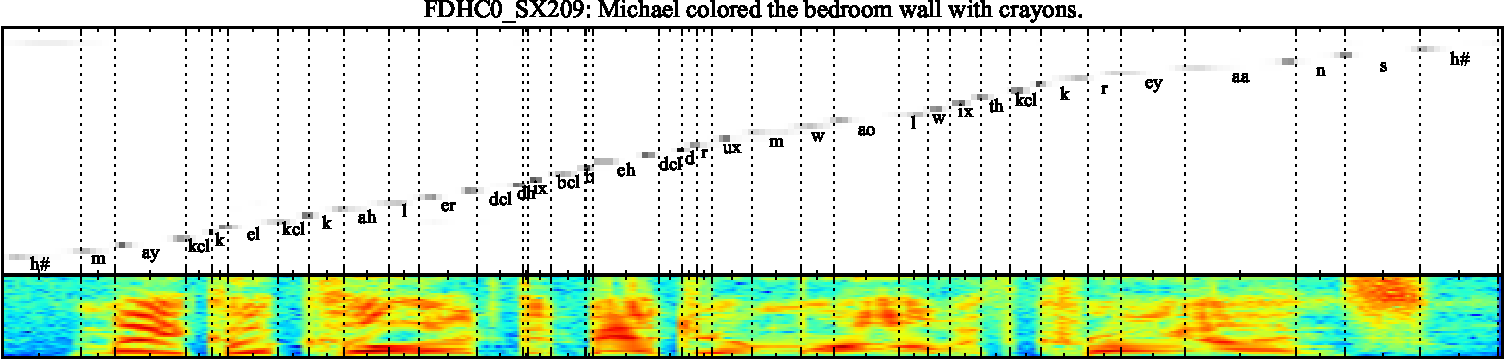
\includegraphics[width=\textwidth]{michael_baseline}

  Convolutional Features
  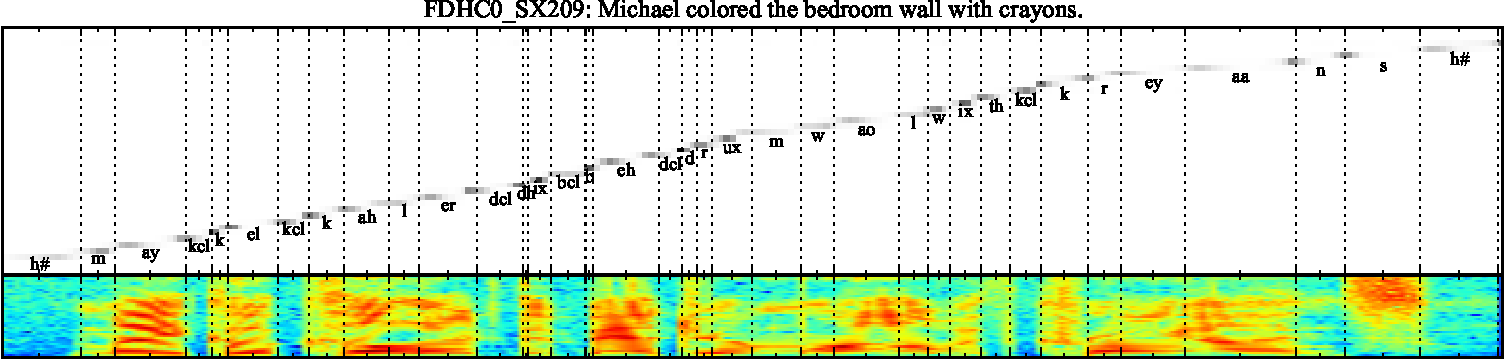
\includegraphics[width=\textwidth]{michael_convfeats}
  Smooth Focus
  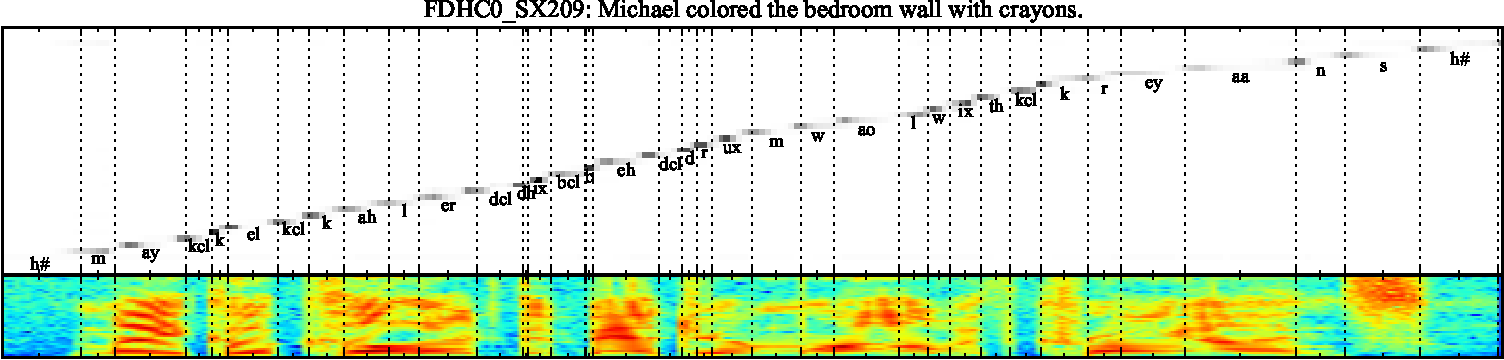
\includegraphics[width=\textwidth]{michael_smooth}
  % \vspace{-.8cm}
  \caption{Alignments
      produced by evaluated models on the FDHC0\_SX209 test utterance. The vertical bars
      indicate ground truth phone location from TIMIT. Each
      row of the upper image indicates frames selected by
      the attention mechanism to emit a phone symbol. Compare with
      Figure 3. in the main text.
  }  

  \vspace{-4mm}
\end{figure}

\begin{figure}[h]
  \centering
  Baseline
  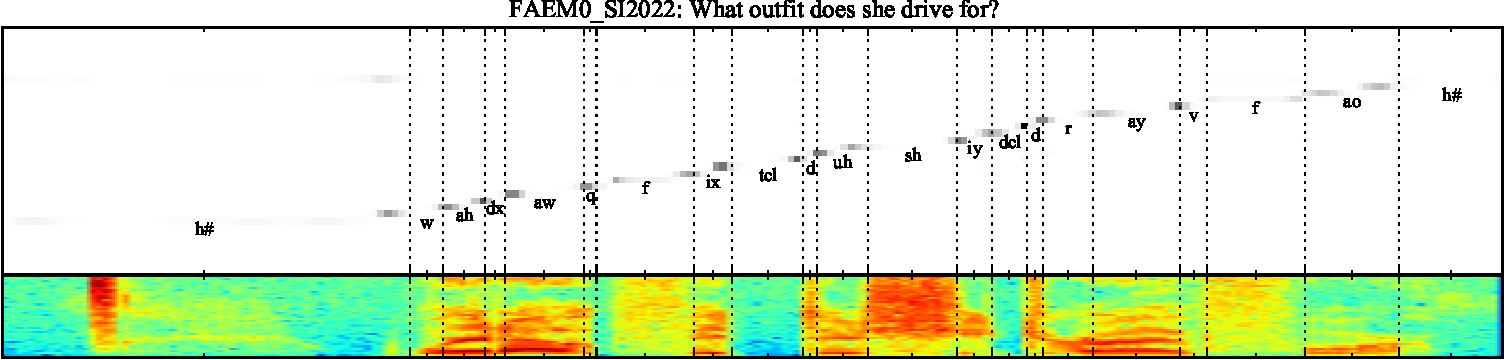
\includegraphics[width=\textwidth]{FAEM0_SI2022_baseline}

  Convolutional Features
  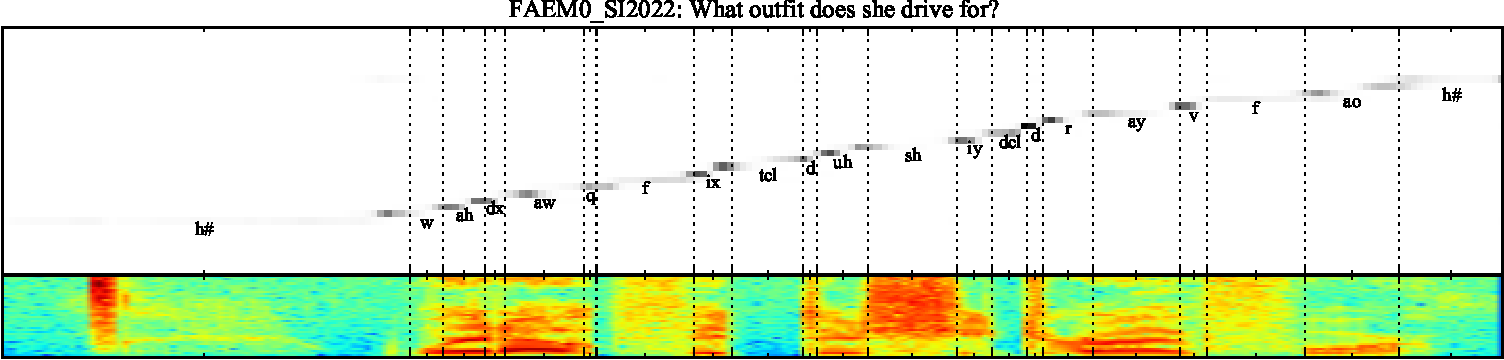
\includegraphics[width=\textwidth]{FAEM0_SI2022_convfeats}
  Smooth Focus
  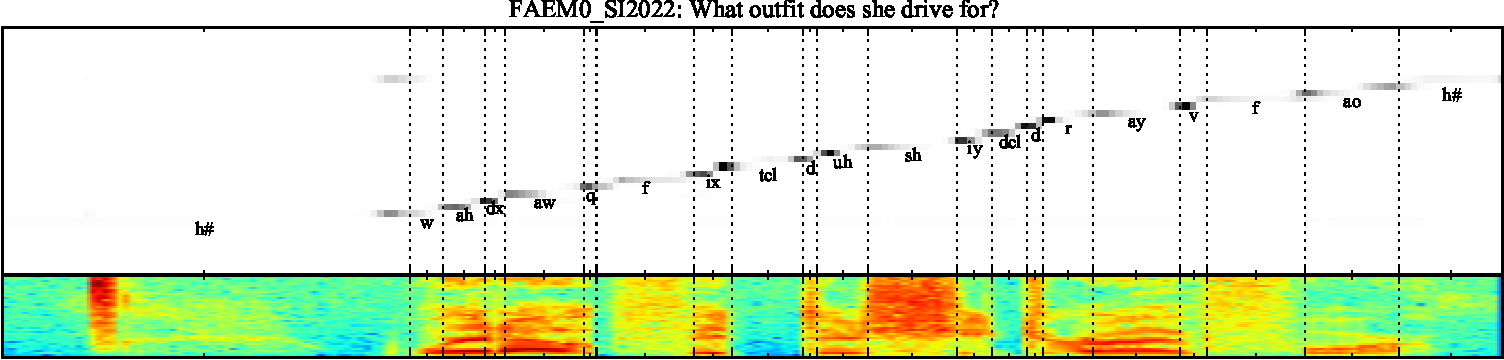
\includegraphics[width=\textwidth]{FAEM0_SI2022_smooth}
  % \vspace{-.8cm}
  \caption{Alignments
      produced by evaluated models on the FAEM0\_SI2022 train utterance. The vertical bars
      indicate ground truth phone location from TIMIT. Each
      row of the upper image indicates frames selected by
      the attention mechanism to emit a phone symbol. Compare with
      Figure 3. in the main text.
  }  

  \vspace{-4mm}
\end{figure}



\begin{figure}[h]
  \centering
  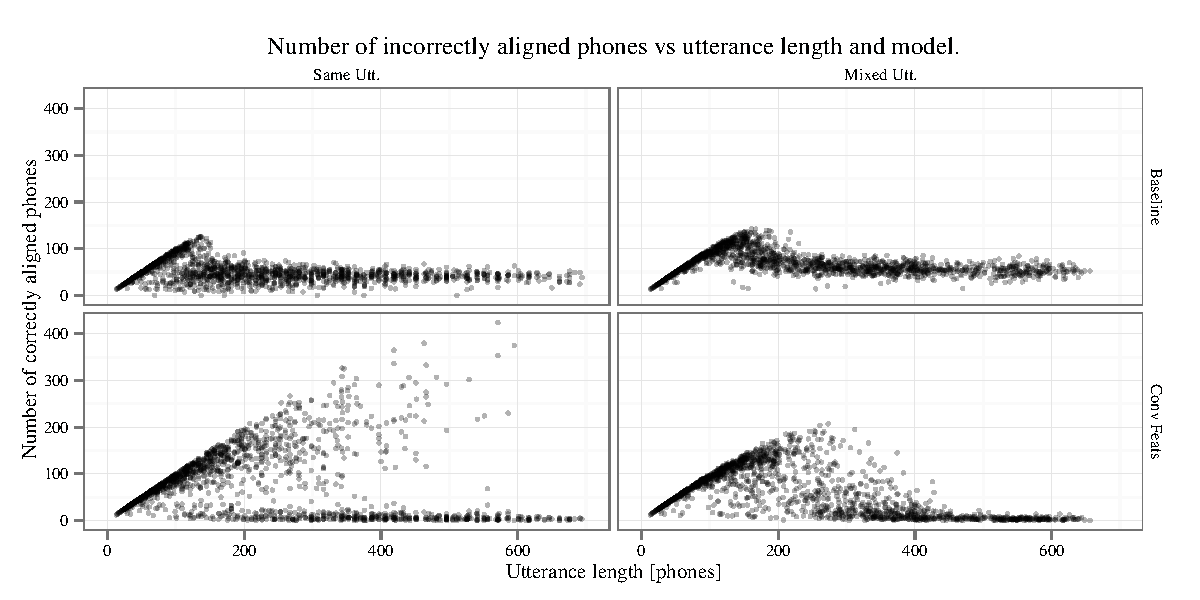
\includegraphics[width=\textwidth]{alis_fails}
  \caption[Results of force-aligning of long utterances.]{Close-up on
    the two failure modes of ARSG. Results of
    force-aligning concatenated TIMIT utterances. Each dot represents
    a single utterance. The left panels show results for
    concatenations of the same utterance. The right panels show
    results for concatenations of randomly chosen utterances. We
    compare the baseline network having a content-based only attention
    mechanism (top row) with a hybrid attention mechanism that uses
    convolutional features (bottom row). While neither model is able
    to properly align long sequences, they fail in different ways: the
    baseline network always aligns about 50 phones, while the
    location-aware network fails to align any phone. Compare with
    Figure 4 form the main paper.}
  %\label{fig:forced_ali_fail}
\end{figure}

\begin{sidewaysfigure}[h]
  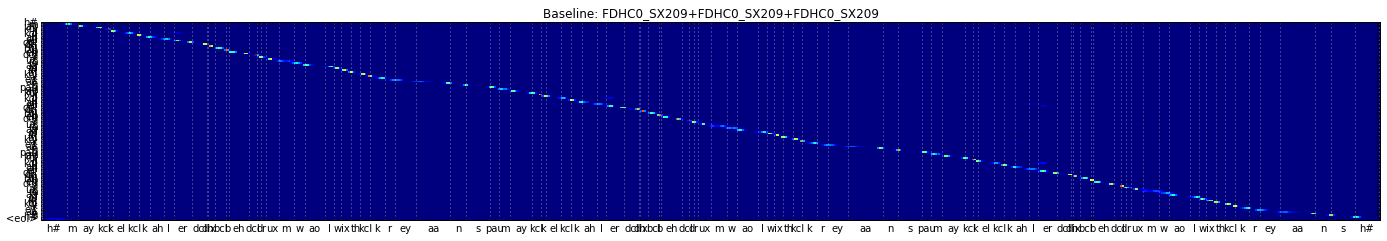
\includegraphics[width=\textwidth]{forced_alignment_baseline_OK_3x_FDHC0_SX209}
  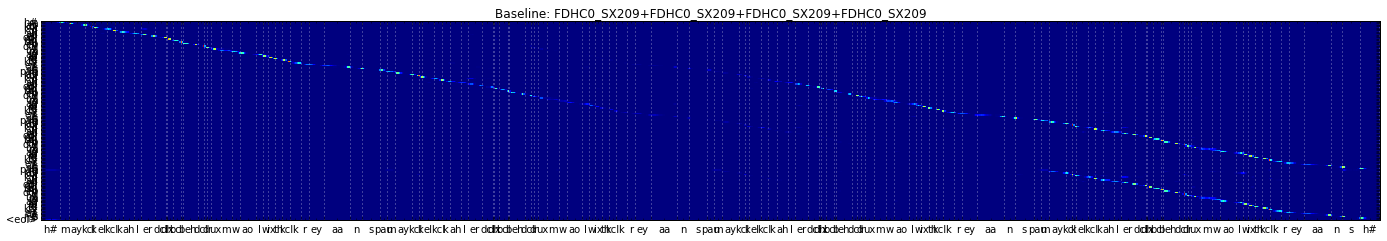
\includegraphics[width=\textwidth]{forced_alignment_baseline_FAIL_4x_FDHC0_SX209}
  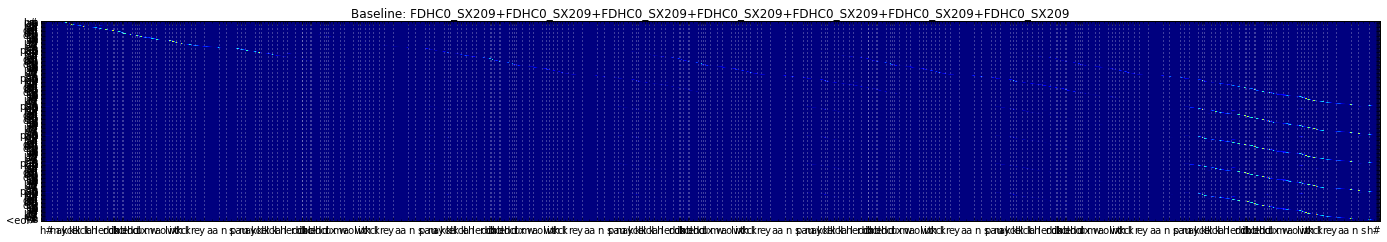
\includegraphics[width=\textwidth]{forced_alignment_baseline_FAIL_7x_FDHC0_SX209}
  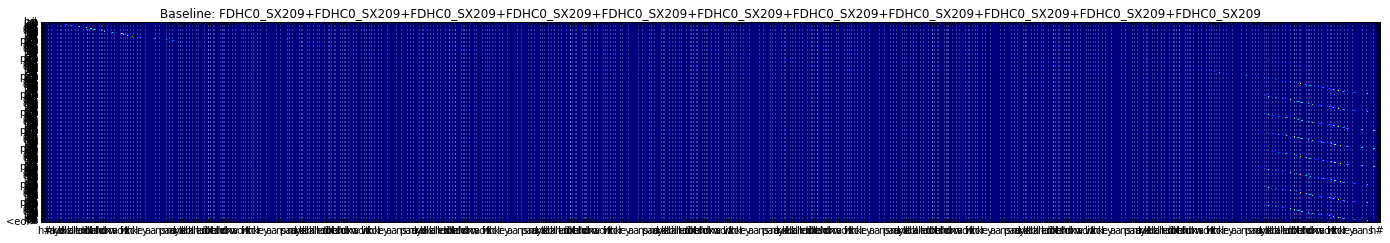
\includegraphics[width=\textwidth]{forced_alignment_baseline_FAIL_11x_FDHC0_SX209}
  \caption{The baseline network fails to align more than 3 repetitions
    of FDHC0\_SX209.}
\end{sidewaysfigure}

\begin{sidewaysfigure}[h]
  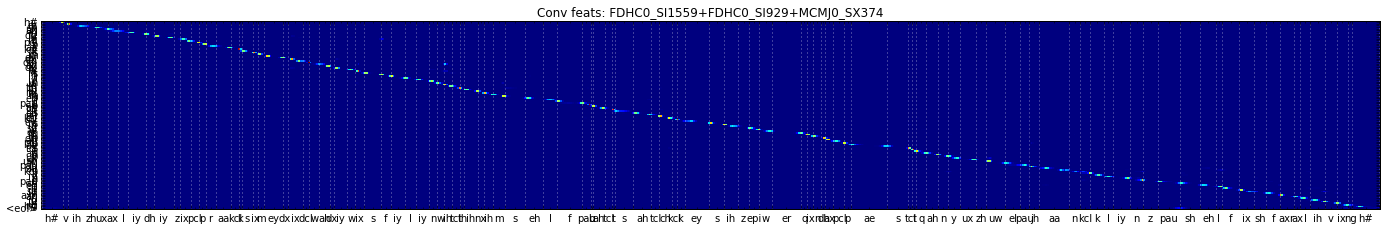
\includegraphics[width=\textwidth]{forced_alignment_baseline_OK_3x_FDHC0_SI1559_MIXED_UTTERANCES}
  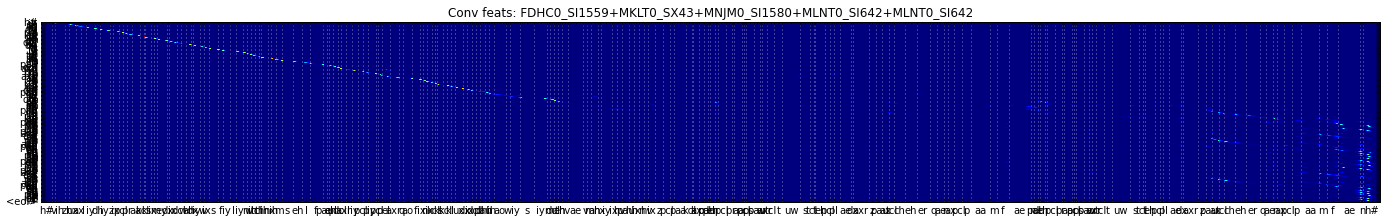
\includegraphics[width=\textwidth]{forced_alignment_baseline_FAIL_5x_FDHC0_SI1559_MIXED_UTTERANCES}
  \caption{The baseline network aligns a concatenation of 3 different
    utterances, but fails to align 5.}
\end{sidewaysfigure}

\begin{sidewaysfigure}[h]
  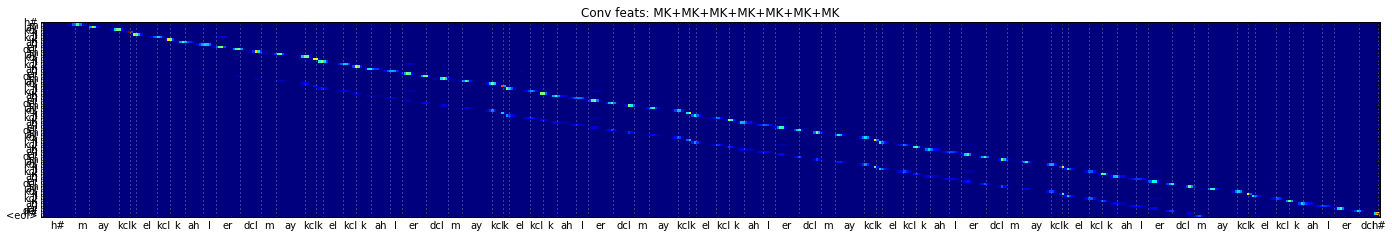
\includegraphics[width=\textwidth]{forced_alignment_baseline_micheal_repeated_with_wondowing}
  \caption{Forced alignment of 7 repetitions of the phrase ``Michael
    colored'' performed with the baseline model with windowing enabled
  (the alignment was constrained to $\pm 75$ frames from the expected
  position of the generator at the last step. The window is wider than
the pattern and the net confuses similar content. Strangely, the first
two repetitions are aligned without any confusion with subsequent ones --
the network starts to confound phoneme location only starting from the
third repetition (as seen by the parallel strand of alignment which
starts when the network starts to emit the phrase for the third time).
}
\end{sidewaysfigure}


\begin{sidewaysfigure}[h]
  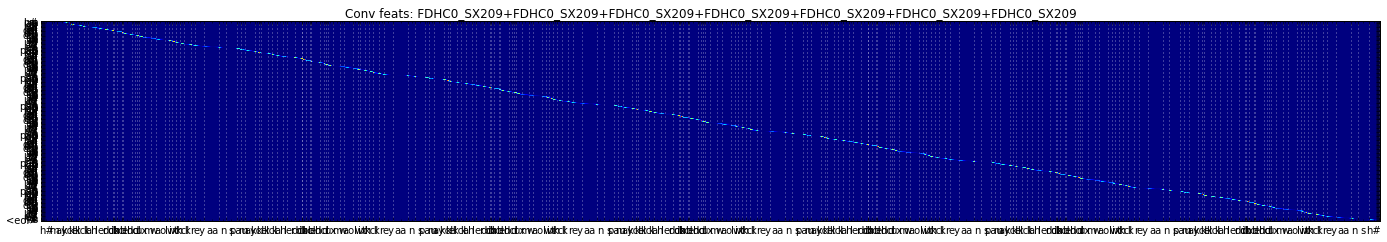
\includegraphics[width=\textwidth]{forced_alignment_convfeats_OK_7x_FDHC0_SX209}
  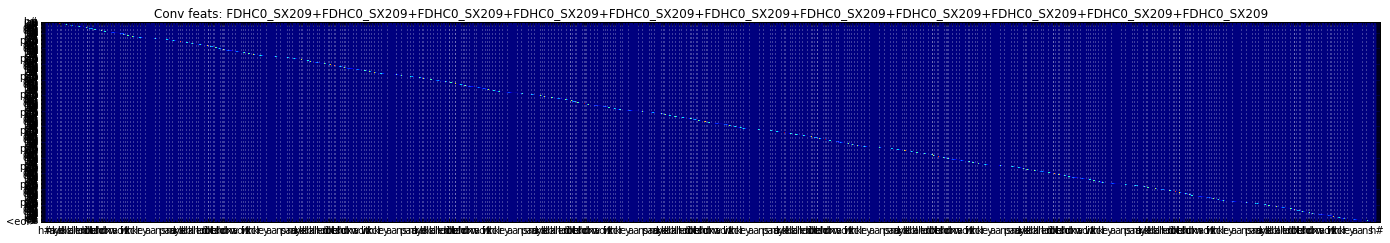
\includegraphics[width=\textwidth]{forced_alignment_convfeats_OK_11x_FDHC0_SX209}
  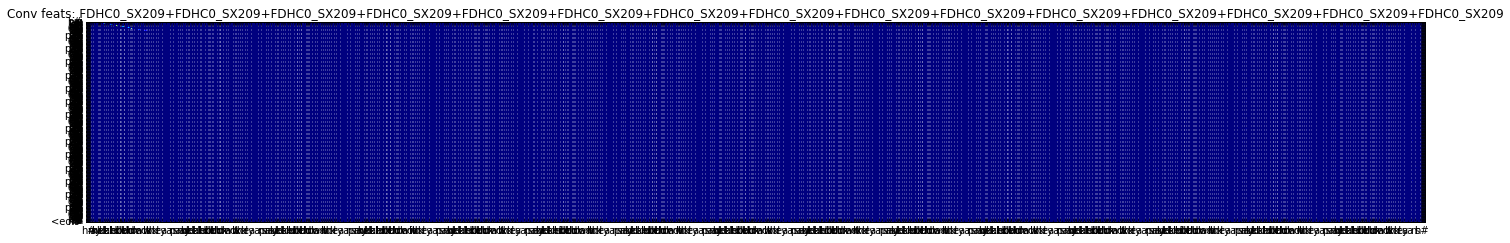
\includegraphics[width=\textwidth]{forced_alignment_convfeats_FAIL_15x_FDHC0_SX209}
  \caption{The location-aware network correctly aligns 7 and 11
    repetitions of FDHC0\_SX209, butfails to align 15 repetitions
    of FDHC0\_SX209.}
\end{sidewaysfigure}

\begin{sidewaysfigure}[h]
  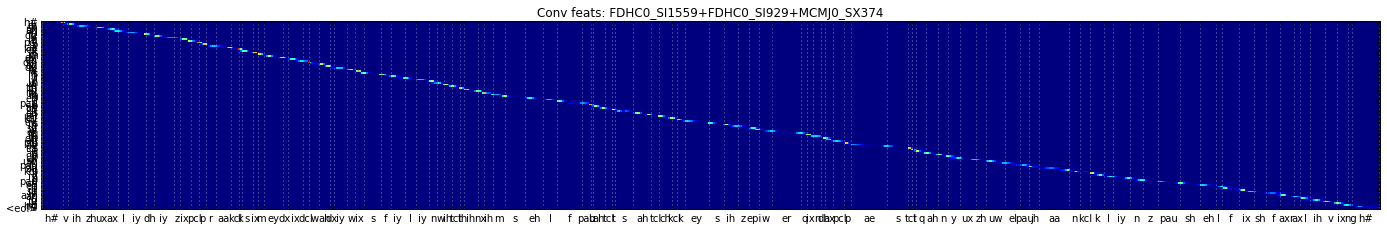
\includegraphics[width=\textwidth]{forced_alignment_convfeats_OK_3x_FDHC0_SI1559_MIXED_UTTERANCES}
  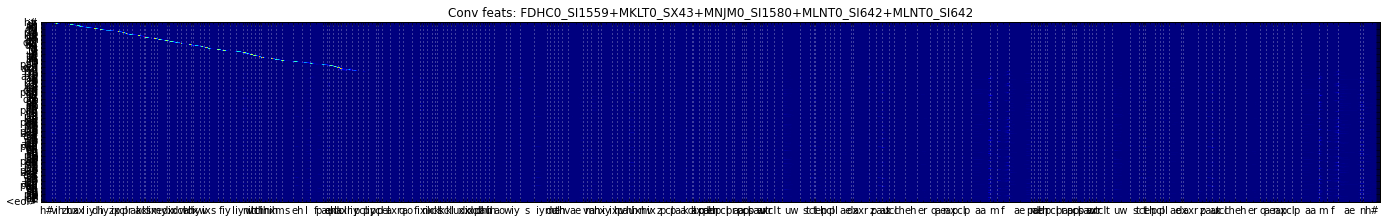
\includegraphics[width=\textwidth]{forced_alignment_convfeats_FAIL_5x_FDHC0_SI1559_MIXED_UTTERNACES}
  \caption{The location-aware network aligns a concatenation of 3 different
    utterances, but fails to align 5.}
\end{sidewaysfigure}

\clearpage
\section{Detailed results of experiments}

\begin{table}[h]
  \centering
  \caption{Phoneme error rates while decoding with various
    modifications. Compare with Figure 5 from the main paper.}
%narrow one without dev errs
% \begin{tabular}{lrrrrrrrr}
% algorithm &   Plain &         &  Keep 1 & Keep 10 & Keep 50 &
% $\beta=2$ & Win. $\pm 75$ & Win. $\pm 150$ \\
% dataset &     dev &    test &    test &    test &    test &    test &       test &        test \\
% Baseline     & $15.9\%$ & $18.7\%$ & $20.2\%$ & $18.7\%$ & $18.7\%$ & $18.9\%$ &    $18.7\%$ &     $18.6\%$ \\
% Conv Feats   & $16.1\%$ & $18.0\%$ & $22.3\%$ & $17.9\%$ & $18.0\%$ & $18.7\%$ &    $18.0\%$ &     $18.0\%$ \\
% Smooth Focus & $15.8\%$ & $17.6\%$ & $24.7\%$ & $18.7\%$ & $17.8\%$ & $18.4\%$ &    $17.7\%$ &     $17.6\%$ \\
% \end{tabular}
\setlength\tabcolsep{5pt}
\begin{tabular}{rl|c|c|c|c|c|c|c}
             &         &   Plain  &  Keep 1  & Keep 10  & Keep 50  &
             $\beta=2$ & Win. $\pm 75$ & Win. $\pm 150$ \\ \hline \hline
\multirow{2}{*}{Baseline} &     dev & $15.9\%$ & $17.6\%$ & $15.9\%$ & $15.9\%$ &   $16.1\%$ &       $15.9\%$ &        $15.9\%$ \\
             &    test & $18.7\%$ & $20.2\%$ & $18.7\%$ & $18.7\%$ &
             $18.9\%$ &       $18.7\%$ &        $18.6\%$ \\ \hline
\multirow{2}{*}{Conv Feats} &     dev & $16.1\%$ & $19.4\%$ & $16.2\%$ & $16.1\%$ &   $16.7\%$ &       $16.0\%$ &        $16.1\%$ \\
             &    test & $18.0\%$ & $22.3\%$ & $17.9\%$ & $18.0\%$ &
             $18.7\%$ &       $18.0\%$ &        $18.0\%$ \\ \hline
\multirow{2}{*}{Smooth Focus} &     dev & $15.8\%$ & $21.6\%$ & $16.5\%$ & $16.1\%$ &   $16.2\%$ &       $16.2\%$ &        $16.0\%$ \\
             &    test & $17.6\%$ & $24.7\%$ & $18.7\%$ & $17.8\%$ &   $18.4\%$ &       $17.7\%$ &        $17.6\%$ \\
\end{tabular}
  \label{tab:decoding_singles}
\end{table}


%{\small
%\bibliographystyle{unsrt}
%\bibliography{paper}
%}
